%!TEX encoding = UTF-8 Unicode
\documentclass[french, a4paper, 12pt, twocolumn, landscape]{article}



%% Langue et compilation

\usepackage[utf8]{inputenc}
\usepackage[T1]{fontenc}
\usepackage[french]{babel}

%% LISTE DES PACKAGES

\usepackage{mathtools}     % package de base pour les maths
\usepackage{amsmath}       % mathematical type-setting
\usepackage{amssymb}       % symbols speciaux pour les maths
\usepackage{textcomp}      % symboles speciaux pour el text
\usepackage{gensymb}       % commandes generiques \degree etc...
\usepackage{tikz}          % package graphique
\usepackage{wrapfig}       % pour entourer a cote d'une figure
\usepackage{color}         % package des couleurs
\usepackage{xcolor}        % autre package pour les couleurs
\usepackage{pgfplots}      % pacakge pour creer des graph
\usepackage{epsfig}        % permet d'inclure des graph en .eps
\usepackage{graphicx}      % arguments dans includegraphics
\usepackage{pdfpages}      % permet d'insérer des pages pdf dans le document
\usepackage{subfig}        % permet de creer des sous-figure
\usepackage{pst-all}       % utile pour certaines figures en pstricks
\usepackage{lipsum}        % package qui permet de faire des essais
\usepackage{array}         % permet de faire des tableaux
\usepackage{multicol}      % plusieurs colonnes sur une page
\usepackage{enumitem}      % pro­vides user con­trol: enumerate, itemize and description
\usepackage{hyperref}      % permet de creer des hyperliens dans le document
\usepackage{lscape}        % permet de mettre une page en mode paysage
\usepackage{lmodern}       % permet d'avoir certains "fonts" de bonen qualite
\usepackage{fancyhdr}      % Permet de mettre des informations en hau et en bas de page      
\usepackage[framemethod=tikz]{mdframed} % breakable frames and coloured boxes
\usepackage[top=1.5cm, bottom=1.5cm, left=2.5cm, right=2.5cm]{geometry} % donne les marges
\usepackage[font=normalsize, labelfont=bf,labelsep=endash, figurename=Fig.]{caption} % permet de changer les legendes des figures
\usepackage{lewis}
\usepackage{bohr}
\usepackage{chemfig}
\usepackage{chemist}

%% LIBRAIRIES

\usetikzlibrary{plotmarks} % librairie pour les graphes
\usetikzlibrary{patterns}  % necessaire pour certaines choses predefinies sur tikz
\usetikzlibrary{shadows}   % ombres des encadres
\usetikzlibrary{backgrounds} % arriere plan des encadres


%% MISE EN PAGE

\pagestyle{fancy}     % Défini le style de la page

\renewcommand{\headrulewidth}{1pt}      % largeur du trait en haut de la page
\fancyhead[L]{Seconde générale}         % info coin haut gauche
\fancyhead[R]{Lycée Jean Guéhenno}  % info coin haut droit

% bas de la page
\renewcommand{\footrulewidth}{1pt}      % largeur du trait en bas de la page
\fancyfoot[L]{G. \bsc{LE DOUDIC}}  % info coin bas gauche
\fancyfoot[R]{TP 4 : Famille chimique}                         % info coin bas droit


\setlength{\columnseprule}{1pt} 
\setlength{\columnsep}{30pt}



%% NOUVELLES COMMANDES 

\DeclareMathOperator{\e}{e} % permet d'ecrire l'exponentielle usuellement


\newcommand{\gap}{\vspace{0.15cm}}   % defini une commande pour sauter des lignes
\renewcommand{\vec}{\overrightarrow} % permet d'avoir une fleche qui recouvre tout le vecteur
\newcommand{\bi}{\begin{itemize}}    % begin itemize
\newcommand{\ei}{\end{itemize}}      % end itemize
\newcommand{\bc}{\begin{center}}     % begin center
\newcommand{\ec}{\end{center}}       % end center
\newcommand\opacity{1}               % opacity 
\pgfsetfillopacity{\opacity}

\newcommand*\Laplace{\mathop{}\!\mathbin\bigtriangleup} % symbole de Laplace

\frenchbsetup{StandardItemLabels=true} % je ne sais plus

\newcommand{\smallO}[1]{\ensuremath{\mathop{}\mathopen{}o\mathopen{}\left(#1\right)}} % petit o

\newcommand{\cit}{\color{blue}\cite} % permet d'avoir les citations de couleur bleues
\newcommand{\bib}{\color{black}\bibitem} % paragraphe biblio en noir et blanc
\newcommand{\bthebiblio}{\color{black} \begin{thebibliography}} % idem necessaire sinon bug a cause de la couleur
\newcommand{\ethebiblio}{\color{black} \end{thebibliography}}   % idem
%%% TIKZ


%% COULEURS 


\definecolor{definitionf}{RGB}{220,252,220}
\definecolor{definitionl}{RGB}{39,123,69}
\definecolor{definitiono}{RGB}{72,148,101}

\definecolor{propositionf}{RGB}{255,216,218}
\definecolor{propositionl}{RGB}{38,38,38}
\definecolor{propositiono}{RGB}{109,109,109}

\definecolor{theof}{RGB}{255,216,218}
\definecolor{theol}{RGB}{160,0,4}
\definecolor{theoo}{RGB}{221,65,100}

\definecolor{avertl}{RGB}{163,92,0}
\definecolor{averto}{RGB}{255,144,0}

\definecolor{histf}{RGB}{241,238,193}

\definecolor{metf}{RGB}{220,230,240}
\definecolor{metl}{RGB}{56,110,165}
\definecolor{meto}{RGB}{109,109,109}


\definecolor{remf}{RGB}{230,240,250}
\definecolor{remo}{RGB}{150,150,150}

\definecolor{exef}{RGB}{240,240,240}

\definecolor{protf}{RGB}{247,228,255}
\definecolor{protl}{RGB}{105,0,203}
\definecolor{proto}{RGB}{174,88,255}

\definecolor{grid}{RGB}{180,180,180}

\definecolor{titref}{RGB}{230,230,230}

\definecolor{vert}{RGB}{23,200,23}

\definecolor{violet}{RGB}{180,0,200}

\definecolor{copper}{RGB}{217, 144, 88}

%% Couleur des ref

\hypersetup{
	colorlinks=true,
	linkcolor=black,
	citecolor=blue,
	urlcolor=black
		   }

%% CADRES


% %%%%%%%%%% DEFINITION
% \newmdenv[tikzsetting={fill=definitionf}, linewidth=2pt, linecolor=definitionl, outerlinewidth=0pt, innertopmargin=5pt, innerbottommargin=5pt, innerleftmargin=5pt, innerrightmargin=5pt, leftmargin=0pt]{definition}

% \newmdenv[ tikzsetting={drop shadow={ shadow xshift=1ex, shadow yshift=-0.5em, fill=definitiono, opacity=1, every shadow } }, outerlinewidth=2pt, outerlinecolor=white, linecolor=white, innertopmargin=0pt, innerbottommargin=0pt, innerleftmargin=0pt, innerrightmargin=0pt]{ombredef}


% %%%%%%%%%% THEOREME

% \newmdenv[tikzsetting={fill=theof}, linewidth=2pt, linecolor=theol, outerlinewidth=0pt, innertopmargin=5pt, innerbottommargin=5pt, innerleftmargin=5pt, innerrightmargin=5pt, leftmargin=0pt]{theo}

% \newmdenv[ tikzsetting={drop shadow={ shadow xshift=1ex, shadow yshift=-0.5em, fill=theoo, opacity=1, every shadow } }, outerlinewidth=2pt, outerlinecolor=white, linecolor=white, innertopmargin=0pt, innerbottommargin=0pt, innerleftmargin=0pt, innerrightmargin=0pt]{ombretheo}


% %%%%%%%%%% METHODE

% \newmdenv[tikzsetting={fill=metf}, linewidth=2pt, linecolor=metl, outerlinewidth=0pt, innertopmargin=5pt, innerbottommargin=5pt, innerleftmargin=5pt, innerrightmargin=5pt, leftmargin=0pt]{met}

% \newmdenv[ tikzsetting={drop shadow={ shadow xshift=1ex, shadow yshift=-0.5em, fill=meto, opacity=1, every shadow } }, outerlinewidth=2pt, outerlinecolor=white, linecolor=white, innertopmargin=0pt, innerbottommargin=0pt, innerleftmargin=0pt, innerrightmargin=0pt]{ombremet}



%%%%%%%%%%% RQ

\newmdenv[tikzsetting={fill=remf}, linewidth=2pt, linecolor=remf, outerlinewidth=0pt, innertopmargin=5pt, innerbottommargin=5pt, innerleftmargin=5pt, innerrightmargin=5pt, leftmargin=0pt]{remarque}

\newmdenv[ tikzsetting={drop shadow={ shadow xshift=1ex, shadow yshift=-0.5em, fill=remo, opacity=1, every shadow } }, outerlinewidth=2pt, outerlinecolor=white, linecolor=white, innertopmargin=0pt, innerbottommargin=0pt, innerleftmargin=0pt, innerrightmargin=0pt]{ombreremarque}

%%%%%%%%%%% Cadre pour le titre

\tikzset{every shadow/.style={opacity=1}}

\global\mdfdefinestyle{doc}{backgroundcolor=white, shadow=true, shadowcolor=propositiono, linewidth=1pt, linecolor=black, shadowsize=5pt}
\global\mdfdefinestyle{titr}{backgroundcolor=metf, shadow=true, shadowcolor=propositiono, linewidth=1pt, linecolor=black, shadowsize=5pt}
\global\mdfdefinestyle{theo}{backgroundcolor=theof, shadow=true, shadowcolor=theoo, linewidth=1pt, linecolor=theol, shadowsize=5pt}
\global\mdfdefinestyle{prop}{backgroundcolor=theof, shadow=true, shadowcolor=propositiono, linewidth=1pt, linecolor=theol, shadowsize=5pt}
\global\mdfdefinestyle{def}{backgroundcolor=definitionf, shadow=true, shadowcolor=definitiono, linewidth=1pt, linecolor=definitionl, shadowsize=5pt}
\global\mdfdefinestyle{histo}{backgroundcolor=histf, shadow=true, shadowcolor=propositiono, linewidth=1pt, linecolor=black, shadowsize=5pt}
\global\mdfdefinestyle{avert}{backgroundcolor=white, shadow=true, shadowcolor=averto, linewidth=1pt, linecolor=avertl, shadowsize=5pt}
\global\mdfdefinestyle{met}{backgroundcolor=metf, shadow=true, shadowcolor=meto, linewidth=1pt, linecolor=metl, shadowsize=5pt}
\global\mdfdefinestyle{rem}{backgroundcolor=metf, shadow=true, shadowcolor=meto, linewidth=1pt, linecolor=metf, shadowsize=5pt}
\global\mdfdefinestyle{exo}{backgroundcolor=exef, shadow=true, shadowcolor=propositiono, linewidth=1pt, linecolor=exef, shadowsize=5pt}
\global\mdfdefinestyle{not}{backgroundcolor=definitionf, shadow=true, shadowcolor=propositiono, linewidth=1pt, linecolor=black, shadowsize=5pt}
\global\mdfdefinestyle{proto}{backgroundcolor=protf, shadow=true, shadowcolor=proto, linewidth=1pt, linecolor=protl, shadowsize=5pt}

%%%%%%
\definecolor{cobalt}{rgb}{0.0, 0.28, 0.67}
\definecolor{applegreen}{rgb}{0.55, 0.71, 0.0}

\usepackage{tcolorbox}
  \tcbuselibrary{most}
  \tcbset{colback=cobalt!5!white,colframe=cobalt!75!black}



\newtcolorbox{definition}[1]{
	colback=applegreen!5!white,
  	colframe=applegreen!65!black,
	fonttitle=\bfseries,
  	title={#1}}
\newtcolorbox{Programme}[1]{
	colback=cobalt!5!white,
  	colframe=cobalt!65!black,
	fonttitle=\bfseries,
  	title={#1}}  

\newtcolorbox{Exercice}[1]{
  colback=cobalt!5!white,
  colframe=cobalt!65!black,
  fonttitle=\bfseries,
  title={#1}}  

  \newtcolorbox{Protocol}[1]{
  colback=cyan!5!white,
  colframe=cyan!65!black,
  fonttitle=\bfseries,
  title={#1}}  

\newtcolorbox{Resultat}[1]{
	colback=theof,%!5!white,
	colframe=theoo!85!black,
  fonttitle=\bfseries,
	title={#1}} 	


\def\width{12}
\def\hauteur{5}

\setlength{\parskip}{0pt}%
\setlength{\parindent}{18pt}


%% MODIFICATION DE CHAPTER  
\makeatletter
\def\@makechapterhead#1{%
  %%%%\vspace*{50\p@}% %%% removed!
  {\parindent \z@ \raggedright \normalfont
    \ifnum \c@secnumdepth >\m@ne
        \huge\bfseries \@chapapp\space \thechapter
        \par\nobreak
        \vskip 20\p@
    \fi
    \interlinepenalty\@M
    \Huge \bfseries #1\par\nobreak
    \vskip 40\p@
  }}
\def\@makeschapterhead#1{%
  %%%%%\vspace*{50\p@}% %%% removed!
  {\parindent \z@ \raggedright
    \normalfont
    \interlinepenalty\@M
    \Huge \bfseries  #1\par\nobreak
    \vskip 40\p@
  }}
  
  \newcommand{\isotope}[3]{%
     \settowidth\@tempdimb{\ensuremath{\scriptstyle#1}}%
     \settowidth\@tempdimc{\ensuremath{\scriptstyle#2}}%
     \ifnum\@tempdimb>\@tempdimc%
         \setlength{\@tempdima}{\@tempdimb}%
     \else%
         \setlength{\@tempdima}{\@tempdimc}%
     \fi%
    \begingroup%
    \ensuremath{^{\makebox[\@tempdima][r]{\ensuremath{\scriptstyle#1}}}_{\makebox[\@tempdima][r]{\ensuremath{\scriptstyle#2}}}\text{#3}}%
    \endgroup%
  }%

\makeatother

\usepackage{eurosym}
\usepackage{colortbl}
\usepackage{setspace}
% 
%%
%% DEBUT DU DOCUMENT
%%
\begin{document}


%%%%%%

\titre{Chapitre 9 : Décrire un mouvement}

\doc{1}{Bulletin officiel}{
\begin{center}
	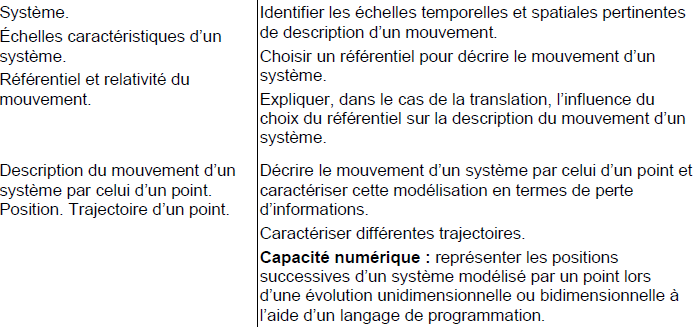
\includegraphics[width=1\textwidth]{BO1.png}
	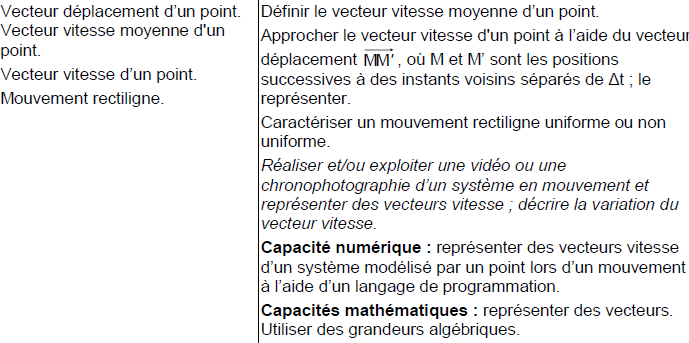
\includegraphics[width=1 \textwidth]{BO2.png}

\end{center}
}

\vspace{1cm}
\doc{2}{Exercices dans le livre scolaire}{
		\begin{enumerate}
			\item Compétence de base : exercice 5,6, 10 page 210
			\item Pour confirmer  : exercice 14, (16, 17,18 au choix) page 211
			\item Parcours expert exercice 20,21 page 213
		\end{enumerate}
}

	\noindent \textbf{Quiz sur la description d'un mouvement}
\begin{center}
	\begin{minipage}{.14\textwidth}
		\centering
		
\includegraphics[width=.5\textwidth]{Quiz1.png}
		
		Quiz 1 - Notion de référentiel : \url{https://forms.office.com/r/uMe5XngTAY?origin=lprLink}
	\end{minipage}\hspace{.5cm}
	\begin{minipage}{.14\textwidth}
		\centering
		
\includegraphics[width=.5\textwidth]{Quiz2.png}

		Quiz 2 - Notion de trajectoire: \url{https://forms.office.com/r/MPtwME5vem?origin=lprLink}
	\end{minipage}\hspace{.5cm}
\begin{minipage}{.14\textwidth}
			\centering
			
\includegraphics[width=.5\textwidth]{Quiz3.png}
	
			Quiz 3 - Le vecteur vitesse : \url{https://forms.office.com/r/g7sZRusPFF?origin=lprLink}
		\end{minipage}
\end{center}


\section*{Introduction}

Ce chapitre aborde la \textbf{mécanique}, c'est à dire le domaine de la physique qui sert à \textbf{décrire} et \textbf{prévoir} le mouvement des objets qui nous entourent, qu'il s'agisse d'une goutte de pluie, d'un car TRANSDEV ou encore des planètes autour du Soleil.

\begin{figure}[ht]
	\centering
	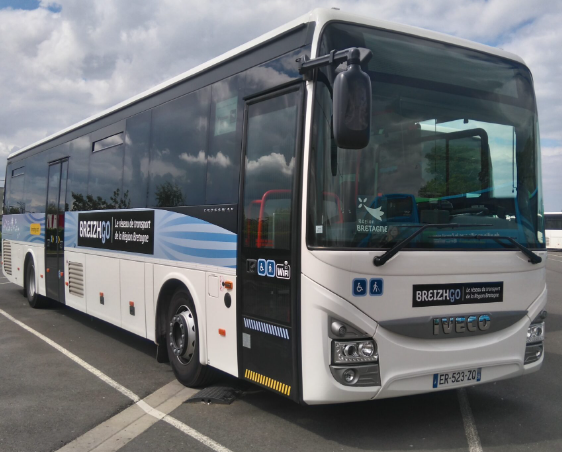
\includegraphics[width=.14\textwidth]{Transdev.png}\hspace{2cm}
	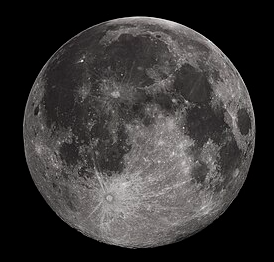
\includegraphics[width=.11\textwidth]{Lune.png}
	\caption{La mécanique permet aussi bien d'étudier le mouvement de la lune autour de la Terre que celui d'un car Breizhgo}
\end{figure}
\clearpage

\section{Système et référentiel}

\begin{definition}{Définition 1 - Système}

		Le système est l'objet ou un ensemble d'objets reliés entre eux, dont on étudie le mouvement.

\end{definition}

En mécanique, on modélise souvent le sytème étudié par \textbf{un point}

\exo{1}{Modéliser des systèmes}{\mobiliser On souhaite étudier le mouvement de la Lune autour de la Terre, représentée sur l'image d'introduction.\textbf{Comment peut-on la modéliser ? Même question pour le bus.}\medskip

\textbf{Solution: } On peut modéliser la lune par son centre de gravité en rotation autour de la Terre fixe avec un repère dont l'origine est au centre de la Terre et trois axes pointant vers trois étoiles lointaines supposées fixes aussi. \medskip

Le bus peut être étudié dans le référentiel terrestre fixe. On pourra étudier le mouvement du bus en le réduisant à son centre de gravité.

}

\subsection{Référentiel}

Pour pouvoir décrire \textbf{la position} d'un système dans l'espace, il faut nécessairement spécifier le \textbf{référentiel} dans lequel on travaille.

\begin{definition}{Définition 2 - Référentiel}

		Le \textbf{référentiel} d'étude est l'objet de référence par rapport auquel on étudie le mouvement du système. On associe au référentiel un \textbf{repère d'espace} (3 directions) et un \textbf{repère de temps} (une horloge). 

\end{definition}

\begin{table}[!ht]
\resizebox{\linewidth}{!}{
	\begin{tabular}{|p{3cm}|p{8cm}|}
	\hline 
	Référentiel  & Repère associé \\ \hline
	 \textbf{Héliocentrique}& \small Origine au centre du Soleil et les axes pointent vers trois étoiles lointaines supposées fixes. \\ \hline
	 \textbf{Géocentrique }& \small Origine au centre de la Terre  et axes orientés vers trois étoiles lointaines supposées fixes. \\ \hline 
	 
	\textbf{Terrestre} & \small Centré sur un objet fixe à la surface de la Terre et axes  liés à la rotation de la Terre. \\ \hline
	\end{tabular}
}
\end{table}

\exo{2}{Référentiels}{On étudie le décollage d'un avion de ligne de type Airbus A320, illustré par les deux images ci-dessous : 
\begin{center}
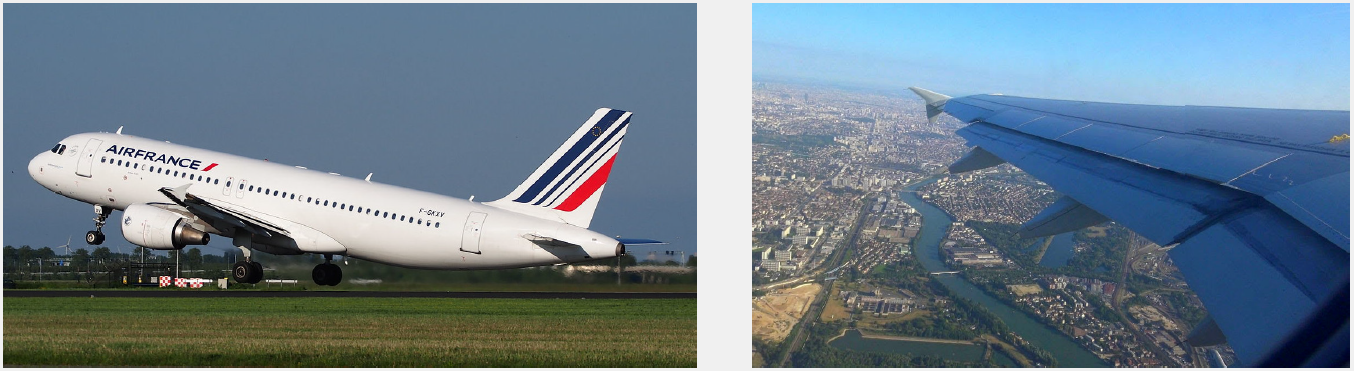
\includegraphics[width=1\textwidth]{Airbus.png}
\end{center}
\begin{enumerate}
	\item \analyser \communiquer Dans quel référentiel est-il pertinent d'étudier le décollage de l'avion ? Pourquoi ?\medskip
	
	\textbf{Il vaut mieux étudier le décollage de l'avion dans le référentiel terrestre lié au sol fixe.}

	\item \analyser Indiquer dans quels référentiels ont été prises les photographies.\medskip
	
	\textbf{Figure de gauche, référentiel terrestre, figure de droite, référetiel  de l'avion entrain de décoller.}

\end{enumerate}
}

	
Le mouvement d'un objet \textbf{dépend donc entièrement de l'observateur} (du référentiel) : on dit que le mouvement est \textbf{relatif}.


\clearpage
\subsection{Trajectoire}

\begin{definition}{Définition 3 - Trajectoire}

	La \textbf{trajectoire} d'un point matériel, dans un référentiel d'étude donné correspond à la courbe formée par l'ensemble des positions successivement occupées par le point matériel lors de son mouvement.

\end{definition}
\bigskip

En particulier, la trajectoire d'un système peut être : 

\begin{itemize}
	\item \textbf{rectiligne} si le système se déplace suivant une \textbf{droite};\medskip
	
	\item \textbf{circulare} si le système se déplace suivant une \textbf{cercle};\medskip
	
	\item \textbf{curviligne} dans tous les autres cas;

\end{itemize}

\begin{figure}[ht]
	\centering
	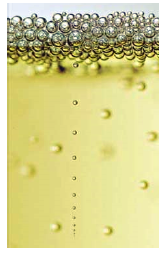
\includegraphics[width=.1\textwidth]{bulles.png}\hspace{.5cm}
	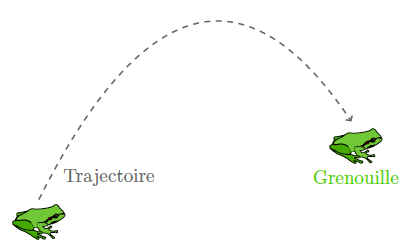
\includegraphics[width=.3\textwidth]{TrajectoireGrenouille.png}
	\caption{\textbf{Chronophotographies}. À gauche des bulles dans un verre de champagne, à droite un saut de grenouille}
\end{figure}
\vspace{3cm}

\exo{3}{Trajectoire}{\analyser La chronophotographie précédente montre l'ascension d'une bulle de champagne. Comment peut-on qualifier sa trajectoire dans le référentiel du verre ? Et dans le cas de la grenouille ? \medskip

\textbf{Solution: } La trajectoire de la bulle de champagne peut être qualifiée de rectiligne accélérée. En effet les différentes positions de la bulles sont de plus en plus espacées ce qui signifie que la vitesse augmente.\medskip

Le saut de la grenouille est une trajectoire curviligne.
}

\subsection{Vecteur déplacement}

Afin de pouvoir décrire le déplacement d'un système d'un point $M$ à un point $M^\prime$, il est commode de définir son \textbf{vecteur déplacement} $\overrightarrow{MM^\prime}$.

\exo{4}{Vecteur déplacement}{\realiser Le schéma de la page précédente montre la trajectoire suivie par une grenouille au cours d’un saut d’un point $M$ à un point $M^\prime$. \textbf{Représenter ces points
sur le schéma ainsi que le vecteur déplacement
$\vec{MM^\prime}$ de la grenouille}.}

\begin{definition}{Définition 4 - Vecteur déplacement}

Le déplacement du point matériel entre les dates $t$ et $t^\prime$ est défini par le vecteur déplacement  $\overrightarrow{MM^\prime}$.  
\end{definition}

\section{Vitesse d'un système}

La vitesse d'un système permet de connaître \textbf{l'évolution de sa position dans le temps}: plus un stème va vite, plus sa position change rapidement.

% \subsection{Vecteur vitesse instantanée}

\subsection{Vecteur vitesse moyenne}\bigskip

\begin{definition}{Définition 5 - Vecteur vitesse moyenne}

		
	Le vecteur vitesse moyenne $\vec{v_i}$, d'un système au point $M_i$ entre deux dates $t$ et $t^\prime$, a pour expression : 

	$$\vec{v_2} = \dfrac{\overrightarrow{M_{1}M_{2}}}{t_{3}-t_{1}}$$

	$M_{3}M_{1}$ la distance entre les points en mètres, $t_{3}-t_{1}$ la durée séparant les instants $t_{3}$ et $t_{1}$ en secondes, $v$ la valeur de la vitesse en mètres par secondes.


\end{definition}\bigskip
\begin{figure}[ht]
	\centering
	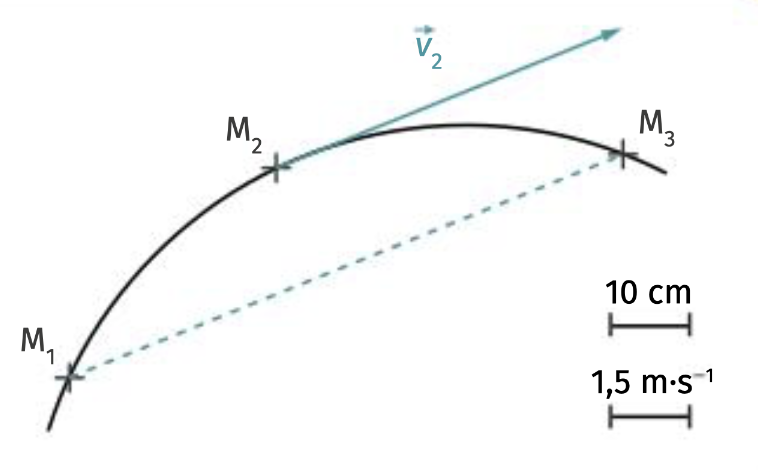
\includegraphics[width=.5\linewidth]{SchemaVecteurVitesse.png}
\end{figure}
\begin{Proposition}{Propriété 1 - Caractéristiques du vecteur vitesse}

		
	Ce vecteur a les caractéristiques suivantes:
	\begin{itemize}
		\item \textbf{direction :} parallèle au segment $M_{1}M_{2}$
		\item \textbf{sens :} celui du mouvement;
		\item \textbf{norme :} $v_2 = \dfrac{M_{1}M_{2}}{t_{3}-t_{1}}.$ Avec $ M_{1}M_{2}$ la distance entre $M_1$ et $M_3$ en mètres. $t_3-t_1$ la durée séparant les instants $t_1$ et $t_3$. $v_2$ la valeur de la vitesse en $m/s$.

	\end{itemize}

\end{Proposition}


\exo{5}{Vitesse moyenne}{On considère le saut de grenouille. La distance $MM^\prime$ est de 0,80 m, et le temps de vol de la grenouille est de $\Delta t =0,3$ secondes.\medskip

\begin{enumerate}
	\item \realiser Calculer la valeur de la vitesse moyenne de la grenouille.\medskip
	
	\textbf{Solution : } Par définition $v = \dfrac{d}{\Delta t} = \dfrac{0,80}{0,3} = 3~\rm m/s$

	\item \realiser \analyser Comment est orienté le vecteur vitesse moyenne ?\medskip
	
	\textbf{Solution:} Le vecteur vitesse moyenne est orientée dans la même direction et sens que le vecteur position $\vec{MM\prime}$
\end{enumerate}}

\section{Vecteur vitesse instantanée}

Le vecteur vitesse moyenne entre deux points ne permet pas de décrire les éventuelles variations de vitesse du système entre ces deux points. Le vecteur \textbf{vitesse instantanée} le permet.

\begin{definition}{Définition 6 - Vecteur vitesse instantanée}

		Pour obtenir la vitesse instantanée du point matériel $M$ à la date $t$, il faut connaître sa position à une date $t^\prime$ très proche de $t$. On calcule alors le vecteur vitesse instantanée : 
	
		$$\vec{v} = \dfrac{\vec{MM^\prime}}{\Delta t}\text{  avec } \Delta t = t^\prime - t$$

\end{definition}

% \begin{Proposition}{Propriété 2 - Vecteur vitesse instantanée}
	
% \end{Proposition}

\end{document}

%%
%% FIN DU DOCUMENT
%%
